\apendice{Documentación de usuario}

\section{Requisitos software y hardware para ejecutar el proyecto}

En este apartado se describen los requisitos mínimos necesarios para ejecutar InteraDD, tanto de forma local como mediante el despliegue realizado en la plataforma Render \cite{render}.

\subsection*{Requisitos hardware}

\begin{itemize}
    \item \textbf{Procesador:} procesador de doble núcleo o superior.
    \item \textbf{Memoria RAM:} al menos 4 GB.
    \item \textbf{Espacio en disco:} se recomienda disponer de un mínimo de 500 MB de espacio libre.
    \item \textbf{Conexión a Internet:} necesaria para la instalación de dependencias y para acceder a la versión desplegada de la aplicación.
\end{itemize}

\subsection*{Requisitos software}

Para utilizar la aplicación desplegada únicamente es necesario disponer de:

\begin{itemize}
    \item \textbf{Sistema operativo:} cualquier sistema operativo compatible con un navegador web moderno.
    \item \textbf{Navegador web:} Google Chrome, Mozilla Firefox, Microsoft Edge o cualquier otro navegador actualizado.
\end{itemize}

En caso de ejecutar la aplicación de forma local, también será necesario disponer de:

\begin{itemize}
    \item \textbf{Python:} versión 3.11 o superior.
    \item \textbf{Git:} recomendado para clonar el repositorio del proyecto.
    \item \textbf{Dependencias del proyecto:} todas las librerías especificadas en el archivo \texttt{requirements.txt}, entre las que destacan:
    \begin{itemize}
        \item \texttt{dash}
        \item \texttt{dash-bootstrap-components} (versión 1.6.0 o superior)
        \item \texttt{pandas}
    \end{itemize}
    \item De forma opcional se puede descargar Anaconda o miniconda para el manejo de los entornos virtuales, lo que se recomienda.
\end{itemize}

\section{Instalación y puesta en marcha}

La aplicación puede utilizarse directamente desde la versión desplegada en Render accediendo a la siguiente dirección:

\begin{center}
\texttt{https://tfg-7z0a.onrender.com/}
\end{center}

No obstante, se recomienda ejecutar InteraDD de forma local. La versión desplegada en Render presenta limitaciones propias del servicio gratuito, como tiempos de inactividad cuando la aplicación no ha sido utilizada durante un periodo prolongado o restricciones en el tiempo de ejecución.
Con el fin de facilitar su ejecución local y garantizar la reproducibilidad del proyecto, se pone a disposición el repositorio de GitHub que contiene el código fuente, la documentación y el resto de recursos necesarios para su instalación y puesta en funcionamiento:
\begin{center}
\texttt{https://github.com/CarmenRu/TFG}
\end{center}

Dado que el desarrollo del proyecto se realizó utilizando \textit{Anaconda}, se recomienda instalar previamente \textit{Anaconda} (o, de forma equivalente, \textit{Miniconda}) para garantizar la compatibilidad del entorno de ejecución.

Una vez instalado, deben seguirse los siguientes pasos.

\begin{enumerate}
    \item Clonar el repositorio del proyecto:

\begin{verbatim}
git clone https://github.com/CarmenRu/TFG
\end{verbatim}

    \item Acceder al directorio del proyecto:

\begin{verbatim}
cd TFG
\end{verbatim}

    \item Crear un entorno virtual con Conda utilizando Python 3.11:

\begin{verbatim}
conda create -n interadd python=3.11
\end{verbatim}

    \item Activar el entorno:

\begin{verbatim}
conda activate interadd
\end{verbatim}

    \item Instalar las dependencias del proyecto:

\begin{verbatim}
pip install -r requirements.txt
\end{verbatim}

    Aunque el entorno se crea con Conda, las dependencias del proyecto se instalan mediante \texttt{pip}, ya que todas ellas se encuentran especificadas en el archivo \texttt{requirements.txt}.

    \item Ejecutar la aplicación:

\begin{verbatim}
python app.py
\end{verbatim}

    \item Abrir en el navegador la dirección mostrada en la terminal, que normalmente será:

\begin{center}
\texttt{http://127.0.0.1:8050/}
\end{center}

\end{enumerate}

Una vez finalizada la utilización de la aplicación, el entorno puede desactivarse mediante el comando:

\begin{verbatim}
conda deactivate
\end{verbatim}

\section{Manual de usuario}

La Figura \ref{fig:inicio} muestra la interfaz principal de InteraDD. En ella se presenta el logotipo de la aplicación junto con una breve descripción de su funcionamiento, proporcionando al usuario una visión general de la herramienta antes de realizar cualquier consulta.

En la parte izquierda de la interfaz se encuentran los campos de selección de los dos principios activos cuya posible interacción farmacológica se desea analizar, así como el botón \textit{Search interaction}, encargado de iniciar el proceso de búsqueda.

Una vez realizada la consulta, se habilitan cuatro funcionalidades adicionales que permiten obtener información complementaria sobre la interacción detectada. Concretamente, el usuario puede consultar las enzimas implicadas en el metabolismo de los principios activos, obtener una explicación del mecanismo responsable de la interacción, visualizar los efectos adversos asociados a cada medicamento y consultar posibles alternativas terapéuticas cuando estas se encuentren disponibles.

\begin{figure}[ht]
    \centering
    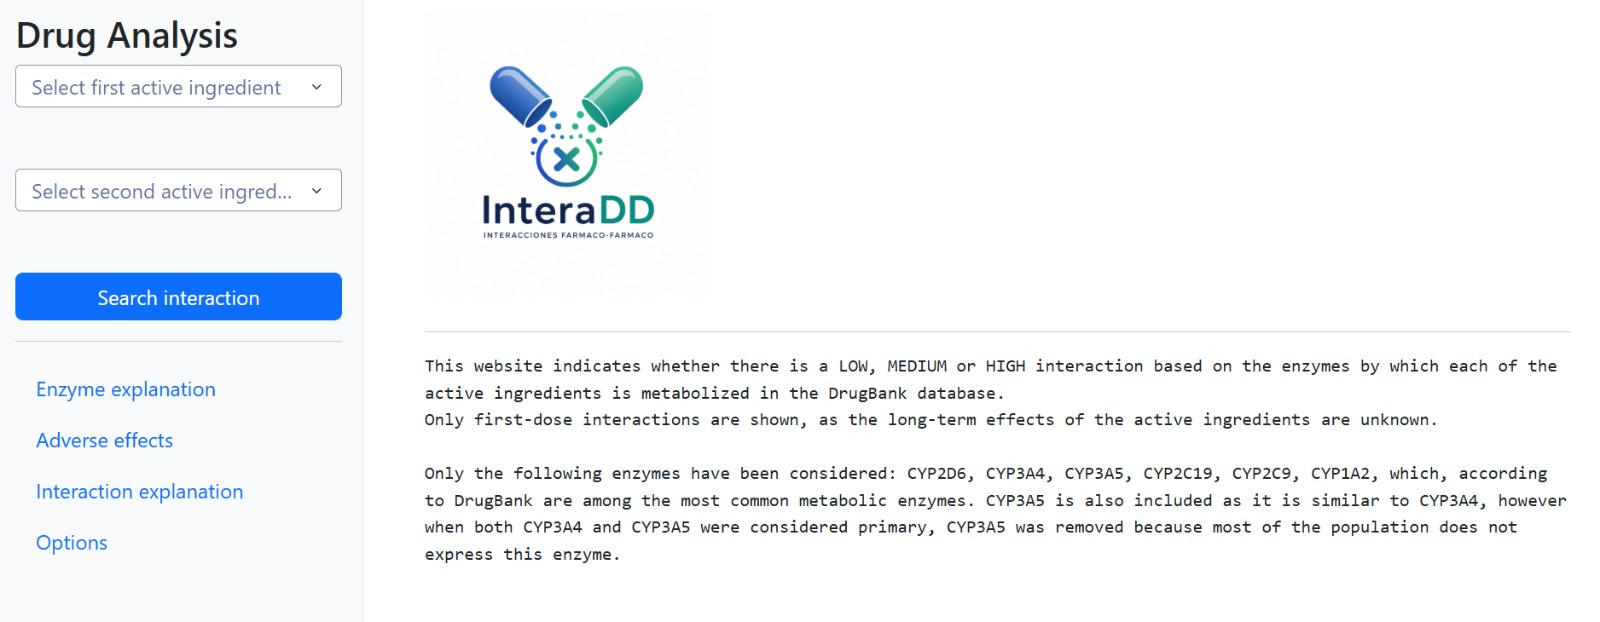
\includegraphics[width=\textwidth]{img/pagina_principal.png}
    \caption{Pantalla principal de InteraDD.}
    \label{fig:inicio}
\end{figure}

\subsection*{Ejemplo de uso: interacción entre clopidogrel y omeprazol}

Para ilustrar el funcionamiento de la aplicación se utilizará el ejemplo formado por los principios activos clopidogrel y omeprazol, una combinación ampliamente conocida por presentar una interacción farmacológica de alta relevancia clínica.

Tras seleccionar ambos principios activos y pulsar el botón \textit{Search interaction}, la aplicación muestra el resultado representado en la Figura \ref{fig:interaccion}. En este caso, la interacción detectada se clasifica como \textit{HIGH}, apareciendo resaltada mediante un recuadro de color rojo. Del mismo modo, las interacciones moderadas y leves se representan mediante los colores amarillo y verde, respectivamente.

Además, la aplicación incorpora un desplegable que explica el motivo de dicha clasificación, indicando las enzimas consideradas como vías metabólicas principales de ambos principios activos.

\begin{figure}[h]
    \centering
    
\includegraphics[width=\textwidth]{img/interaccion.png}
    \caption{Resultado obtenido mediante el botón \textit{Search interaction}.}
    \label{fig:interaccion}
\end{figure}

Una vez obtenida la interacción, el usuario puede acceder al resto de funcionalidades de la aplicación.

\subsubsection*{Botón \textit{Enzyme explanation}}

Esta opción, visible en la Figura \ref{fig:enzimas}, proporciona una explicación detallada de las enzimas implicadas en el metabolismo de cada principio activo. Además, identifica cuáles de ellas han sido consideradas como principales durante el cálculo de la interacción. Cuando un principio activo no presenta una enzima principal o no es metabolizado por ninguna de las enzimas consideradas en el proyecto, esta circunstancia también se indica explícitamente.

\begin{figure}[h]
    \centering
    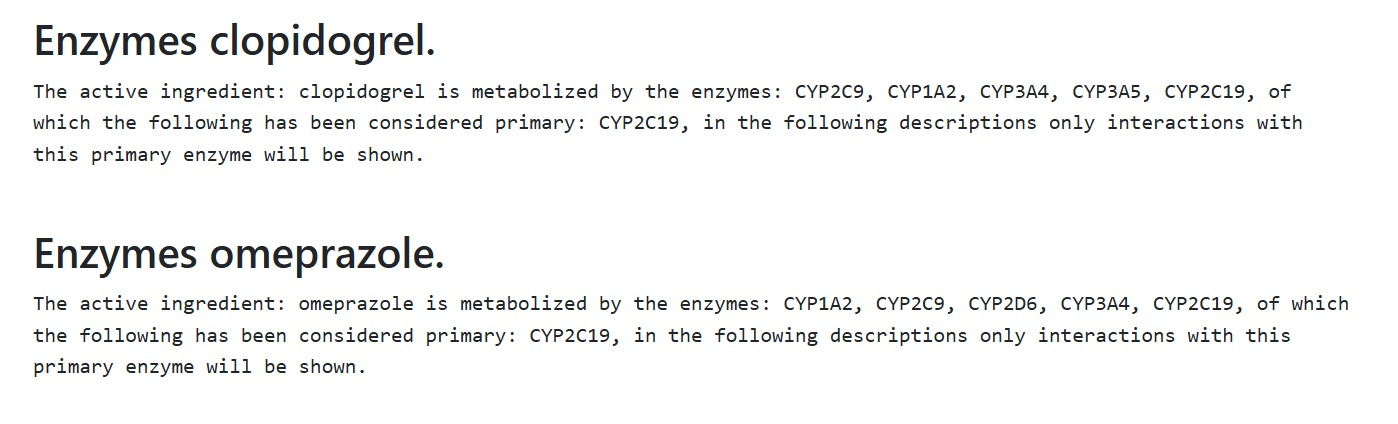
\includegraphics[width=\textwidth]{img/exp_enz.png}
    \caption{Información proporcionada por el botón \textit{Enzyme explanation}.}
    \label{fig:enzimas}
\end{figure}

\subsubsection*{Botón \textit{Adverse effects}}

Esta funcionalidad, que podemos observar en la Figura \ref{fig:grafico_ea} muestra diagramas de barras con los efectos adversos registrados en la base de datos SIDER para cada medicamento, junto con el porcentaje de aparición asociado a cada uno de ellos. Cuando un principio activo dispone de varios códigos de referencia \footnote{Los códigos de referencia son derivados de los códigos ATC de cada medicamento, incluyen de 2 a 5 letras y números que representan la funcionalidad clínica de los fármacos.}, la información se presenta de forma independiente para cada uno de ellos. 

\begin{figure}[h]
    \centering
    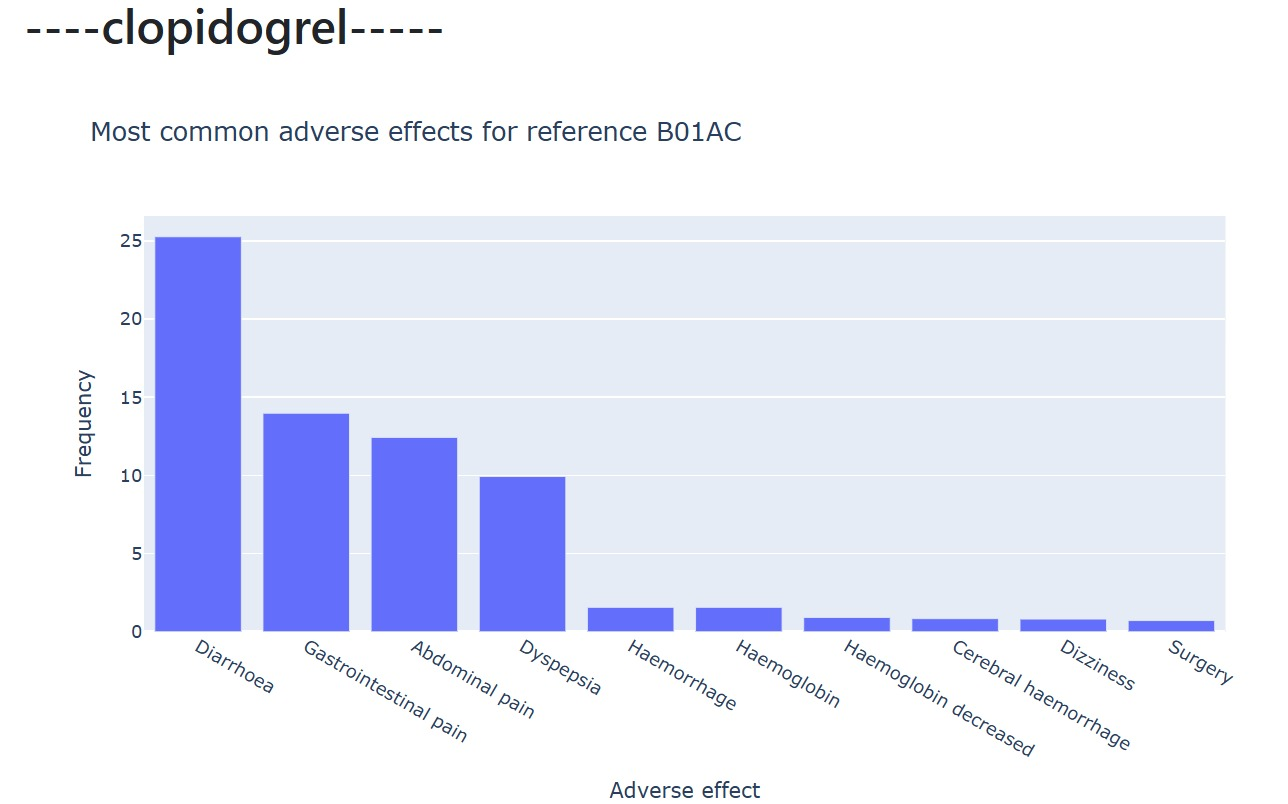
\includegraphics[width=0.85\textwidth]{img/diagrama_ea.png}
    \caption{Diagrama de barras generado mediante el botón \textit{Adverse effects}.}
    \label{fig:grafico_ea}
\end{figure}

\subsubsection*{Botón \textit{Interaction explanation}}

Esta opción, visible en la Figura \ref{fig:acciones} describe el mecanismo responsable de la interacción detectada, indicando el papel que desempeñan las enzimas implicadas sobre cada principio activo. En particular, se especifica si cada fármaco actúa como sustrato, inhibidor o inductor de dichas enzimas y cómo estas acciones afectan a su metabolismo.

\begin{figure}[h]
    \centering
    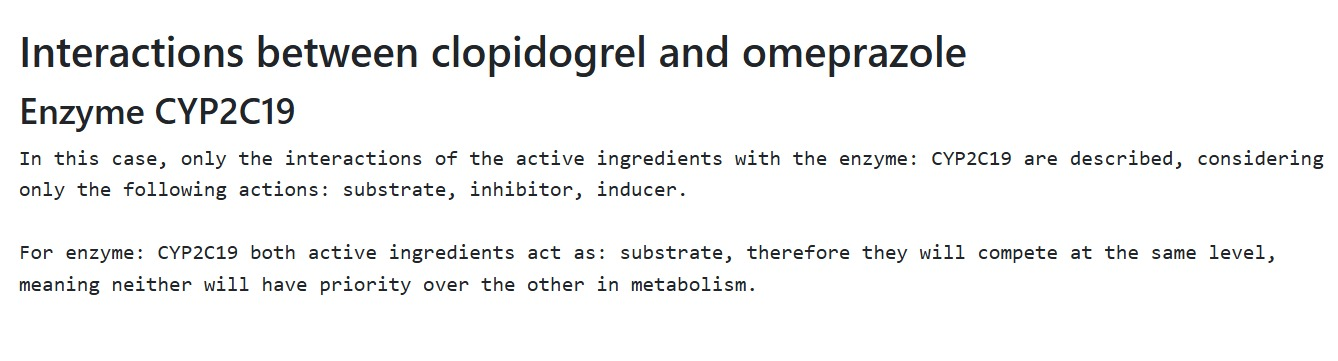
\includegraphics[width=0.85\textwidth]{img/exp_acciones.png}
    \caption{Información mostrada por el botón \textit{Interaction explanation}.}
    \label{fig:acciones}
\end{figure}

\subsubsection*{Botón \textit{Search for drug alternatives}}

Esta funcionalidad muestra las alternativas terapéuticas disponibles para cada uno de los principios activos, obtenidas a partir de sus correspondientes códigos ATC.

A continuación, la aplicación presenta las combinaciones de medicamentos consideradas seguras cuando únicamente se sustituye uno de los principios activos originales, se muestran dichos resultados en la Figura \ref{fig:alternativas}. Finalmente, también se muestran otras combinaciones seguras que no incluyen ninguno de los dos principios activos inicialmente seleccionados.

\begin{figure}[h]
    \centering
    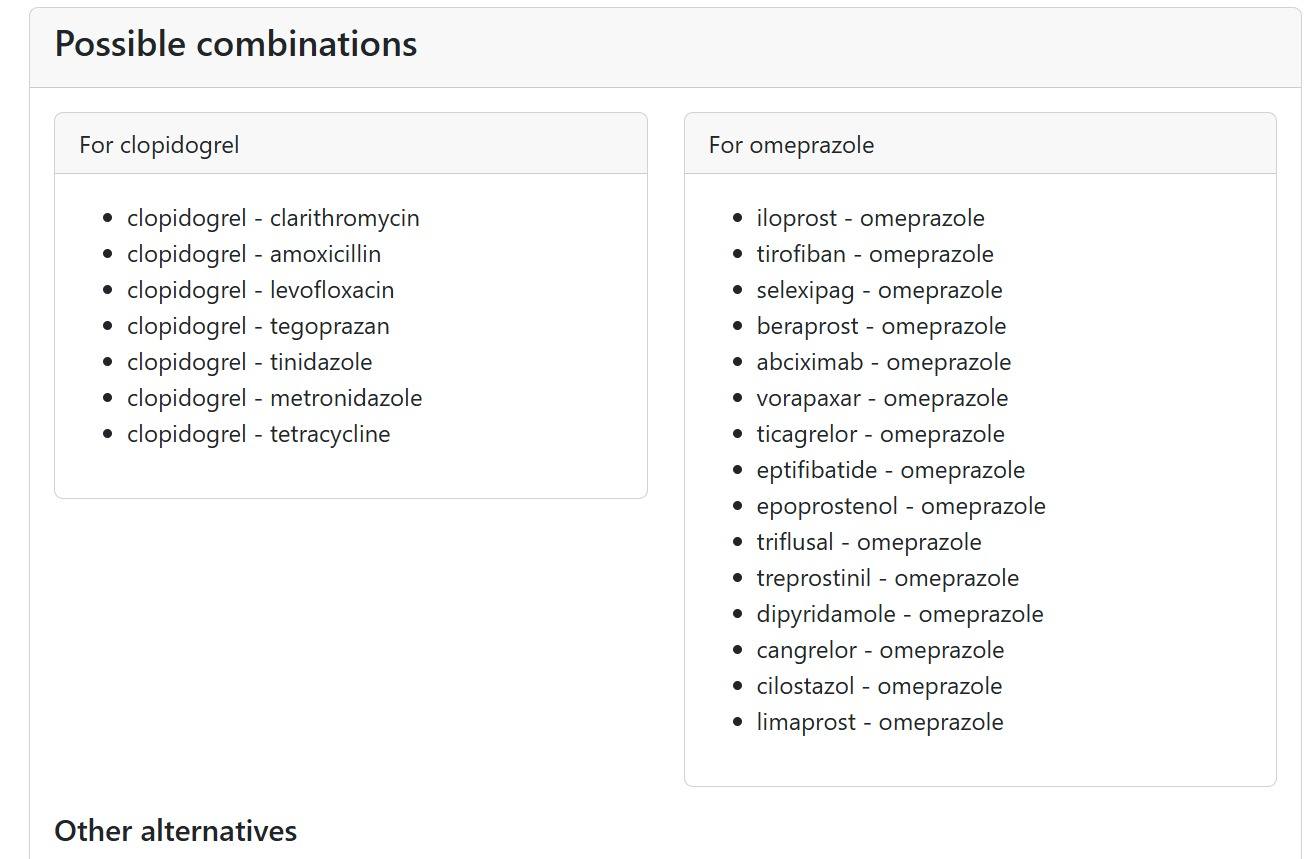
\includegraphics[width=0.85\textwidth]{img/opciones.png}
    \caption{Alternativas terapéuticas propuestas por el botón \textit{Search for drug alternatives}.}
    \label{fig:alternativas}
\end{figure}